\documentclass[12pt,journal]{IEEEtran}
%
% If IEEEtran.cls has not been installed into the LaTeX system files,
% manually specify the path to it like:
% \documentclass[journal]{../sty/IEEEtran}

% *** MISC UTILITY PACKAGES ***
%
%\usepackage{ifpdf}
% Heiko Oberdiek's ifpdf.sty is very useful if you need conditional
% compilation based on whether the output is pdf or dvi.
% usage:
% \ifpdf
%   % pdf code
% \else
%   % dvi code
% \fi
% The latest version of ifpdf.sty can be obtained from:
% http://www.ctan.org/tex-archive/macros/latex/contrib/oberdiek/
% Also, note that IEEEtran.cls V1.7 and later provides a builtin
% \ifCLASSINFOpdf conditional that works the same way.
% When switching from latex to pdflatex and vice-versa, the compiler may
% have to be run twice to clear warning/error messages.

% *** CITATION PACKAGES ***
%
%\usepackage{cite}
% cite.sty was written by Donald Arseneau
% V1.6 and later of IEEEtran pre-defines the format of the cite.sty package
% \cite{} output to follow that of IEEE. Loading the cite package will
% result in citation numbers being automatically sorted and properly
% "compressed/ranged". e.g., [1], [9], [2], [7], [5], [6] without using
% cite.sty will become [1], [2], [5]--[7], [9] using cite.sty. cite.sty's
% \cite will automatically add leading space, if needed. Use cite.sty's
% noadjust option (cite.sty V3.8 and later) if you want to turn this off
% such as if a citation ever needs to be enclosed in parenthesis.
% cite.sty is already installed on most LaTeX systems. Be sure and use
% version 5.0 (2009-03-20) and later if using hyperref.sty.
% The latest version can be obtained at:
% http://www.ctan.org/tex-archive/macros/latex/contrib/cite/
% The documentation is contained in the cite.sty file itself.


\usepackage{color}
\usepackage{listings}
\usepackage{fancyvrb}
\usepackage{hyperref}



% *** GRAPHICS RELATED PACKAGES ***
%
\ifCLASSINFOpdf
   \usepackage[pdftex]{graphicx}
  % declare the path(s) where your graphic files are
  % \graphicspath{{../pdf/}{../jpeg/}}
  % and their extensions so you won't have to specify these with
  % every instance of \includegraphics
  % \DeclareGraphicsExtensions{.pdf,.jpeg,.png}
\else
  % or other class option (dvipsone, dvipdf, if not using dvips). graphicx
  % will default to the driver specified in the system graphics.cfg if no
  % driver is specified.
   \usepackage[dvips]{graphicx}
  % declare the path(s) where your graphic files are
  % \graphicspath{{../eps/}}
  % and their extensions so you won't have to specify these with
  % every instance of \includegraphics
  % \DeclareGraphicsExtensions{.eps}
\fi
% graphicx was written by David Carlisle and Sebastian Rahtz. It is
% required if you want graphics, photos, etc. graphicx.sty is already
% installed on most LaTeX systems. The latest version and documentation
% can be obtained at: 
% http://www.ctan.org/tex-archive/macros/latex/required/graphics/
% Another good source of documentation is "Using Imported Graphics in
% LaTeX2e" by Keith Reckdahl which can be found at:
% http://www.ctan.org/tex-archive/info/epslatex/
%
% latex, and pdflatex in dvi mode, support graphics in encapsulated
% postscript (.eps) format. pdflatex in pdf mode supports graphics
% in .pdf, .jpeg, .png and .mps (metapost) formats. Users should ensure
% that all non-photo figures use a vector format (.eps, .pdf, .mps) and
% not a bitmapped formats (.jpeg, .png). IEEE frowns on bitmapped formats
% which can result in "jaggedy"/blurry rendering of lines and letters as
% well as large increases in file sizes.
%
% You can find documentation about the pdfTeX application at:
% http://www.tug.org/applications/pdftex





% *** MATH PACKAGES ***
%
%\usepackage[cmex10]{amsmath}
% A popular package from the American Mathematical Society that provides
% many useful and powerful commands for dealing with mathematics. If using
% it, be sure to load this package with the cmex10 option to ensure that
% only type 1 fonts will utilized at all point sizes. Without this option,
% it is possible that some math symbols, particularly those within
% footnotes, will be rendered in bitmap form which will result in a
% document that can not be IEEE Xplore compliant!
%
% Also, note that the amsmath package sets \interdisplaylinepenalty to 10000
% thus preventing page breaks from occurring within multiline equations. Use:
%\interdisplaylinepenalty=2500
% after loading amsmath to restore such page breaks as IEEEtran.cls normally
% does. amsmath.sty is already installed on most LaTeX systems. The latest
% version and documentation can be obtained at:
% http://www.ctan.org/tex-archive/macros/latex/required/amslatex/math/





% *** SPECIALIZED LIST PACKAGES ***
%
%\usepackage{algorithmic}
% algorithmic.sty was written by Peter Williams and Rogerio Brito.
% This package provides an algorithmic environment fo describing algorithms.
% You can use the algorithmic environment in-text or within a figure
% environment to provide for a floating algorithm. Do NOT use the algorithm
% floating environment provided by algorithm.sty (by the same authors) or
% algorithm2e.sty (by Christophe Fiorio) as IEEE does not use dedicated
% algorithm float types and packages that provide these will not provide
% correct IEEE style captions. The latest version and documentation of
% algorithmic.sty can be obtained at:
% http://www.ctan.org/tex-archive/macros/latex/contrib/algorithms/
% There is also a support site at:
% http://algorithms.berlios.de/index.html
% Also of interest may be the (relatively newer and more customizable)
% algorithmicx.sty package by Szasz Janos:
% http://www.ctan.org/tex-archive/macros/latex/contrib/algorithmicx/




% *** ALIGNMENT PACKAGES ***
%
%\usepackage{array}
% Frank Mittelbach's and David Carlisle's array.sty patches and improves
% the standard LaTeX2e array and tabular environments to provide better
% appearance and additional user controls. As the default LaTeX2e table
% generation code is lacking to the point of almost being broken with
% respect to the quality of the end results, all users are strongly
% advised to use an enhanced (at the very least that provided by array.sty)
% set of table tools. array.sty is already installed on most systems. The
% latest version and documentation can be obtained at:
% http://www.ctan.org/tex-archive/macros/latex/required/tools/


% IEEEtran contains the IEEEeqnarray family of commands that can be used to
% generate multiline equations as well as matrices, tables, etc., of high
% quality.




% *** SUBFIGURE PACKAGES ***
%\ifCLASSOPTIONcompsoc
%  \usepackage[caption=false,font=normalsize,labelfont=sf,textfont=sf]{subfig}
%\else
%  \usepackage[caption=false,font=footnotesize]{subfig}
%\fi
% subfig.sty, written by Steven Douglas Cochran, is the modern replacement
% for subfigure.sty, the latter of which is no longer maintained and is
% incompatible with some LaTeX packages including fixltx2e. However,
% subfig.sty requires and automatically loads Axel Sommerfeldt's caption.sty
% which will override IEEEtran.cls' handling of captions and this will result
% in non-IEEE style figure/table captions. To prevent this problem, be sure
% and invoke subfig.sty's "caption=false" package option (available since
% subfig.sty version 1.3, 2005/06/28) as this is will preserve IEEEtran.cls
% handling of captions.
% Note that the Computer Society format requires a larger sans serif font
% than the serif footnote size font used in traditional IEEE formatting
% and thus the need to invoke different subfig.sty package options depending
% on whether compsoc mode has been enabled.
%
% The latest version and documentation of subfig.sty can be obtained at:
% http://www.ctan.org/tex-archive/macros/latex/contrib/subfig/




% *** FLOAT PACKAGES ***
%
%\usepackage{fixltx2e}
% fixltx2e, the successor to the earlier fix2col.sty, was written by
% Frank Mittelbach and David Carlisle. This package corrects a few problems
% in the LaTeX2e kernel, the most notable of which is that in current
% LaTeX2e releases, the ordering of single and double column floats is not
% guaranteed to be preserved. Thus, an unpatched LaTeX2e can allow a
% single column figure to be placed prior to an earlier double column
% figure. The latest version and documentation can be found at:
% http://www.ctan.org/tex-archive/macros/latex/base/


%\usepackage{stfloats}
% stfloats.sty was written by Sigitas Tolusis. This package gives LaTeX2e
% the ability to do double column floats at the bottom of the page as well
% as the top. (e.g., "\begin{figure*}[!b]" is not normally possible in
% LaTeX2e). It also provides a command:
%\fnbelowfloat
% to enable the placement of footnotes below bottom floats (the standard
% LaTeX2e kernel puts them above bottom floats). This is an invasive package
% which rewrites many portions of the LaTeX2e float routines. It may not work
% with other packages that modify the LaTeX2e float routines. The latest
% version and documentation can be obtained at:
% http://www.ctan.org/tex-archive/macros/latex/contrib/sttools/
% Do not use the stfloats baselinefloat ability as IEEE does not allow
% \baselineskip to stretch. Authors submitting work to the IEEE should note
% that IEEE rarely uses double column equations and that authors should try
% to avoid such use. Do not be tempted to use the cuted.sty or midfloat.sty
% packages (also by Sigitas Tolusis) as IEEE does not format its papers in
% such ways.
% Do not attempt to use stfloats with fixltx2e as they are incompatible.
% Instead, use Morten Hogholm'a dblfloatfix which combines the features
% of both fixltx2e and stfloats:
%
% \usepackage{dblfloatfix}
% The latest version can be found at:
% http://www.ctan.org/tex-archive/macros/latex/contrib/dblfloatfix/




%\ifCLASSOPTIONcaptionsoff
%  \usepackage[nomarkers]{endfloat}
% \let\MYoriglatexcaption\caption
% \renewcommand{\caption}[2][\relax]{\MYoriglatexcaption[#2]{#2}}
%\fi
% endfloat.sty was written by James Darrell McCauley, Jeff Goldberg and 
% Axel Sommerfeldt. This package may be useful when used in conjunction with 
% IEEEtran.cls'  captionsoff option. Some IEEE journals/societies require that
% submissions have lists of figures/tables at the end of the paper and that
% figures/tables without any captions are placed on a page by themselves at
% the end of the document. If needed, the draftcls IEEEtran class option or
% \CLASSINPUTbaselinestretch interface can be used to increase the line
% spacing as well. Be sure and use the nomarkers option of endfloat to
% prevent endfloat from "marking" where the figures would have been placed
% in the text. The two hack lines of code above are a slight modification of
% that suggested by in the endfloat docs (section 8.4.1) to ensure that
% the full captions always appear in the list of figures/tables - even if
% the user used the short optional argument of \caption[]{}.
% IEEE papers do not typically make use of \caption[]'s optional argument,
% so this should not be an issue. A similar trick can be used to disable
% captions of packages such as subfig.sty that lack options to turn off
% the subcaptions:
% For subfig.sty:
% \let\MYorigsubfloat\subfloat
% \renewcommand{\subfloat}[2][\relax]{\MYorigsubfloat[]{#2}}
% However, the above trick will not work if both optional arguments of
% the \subfloat command are used. Furthermore, there needs to be a
% description of each subfigure *somewhere* and endfloat does not add
% subfigure captions to its list of figures. Thus, the best approach is to
% avoid the use of subfigure captions (many IEEE journals avoid them anyway)
% and instead reference/explain all the subfigures within the main caption.
% The latest version of endfloat.sty and its documentation can obtained at:
% http://www.ctan.org/tex-archive/macros/latex/contrib/endfloat/
%
% The IEEEtran \ifCLASSOPTIONcaptionsoff conditional can also be used
% later in the document, say, to conditionally put the References on a 
% page by themselves.




% *** PDF, URL AND HYPERLINK PACKAGES ***
%
%\usepackage{url}
% url.sty was written by Donald Arseneau. It provides better support for
% handling and breaking URLs. url.sty is already installed on most LaTeX
% systems. The latest version and documentation can be obtained at:
% http://www.ctan.org/tex-archive/macros/latex/contrib/url/
% Basically, \url{my_url_here}.




% *** Do not adjust lengths that control margins, column widths, etc. ***
% *** Do not use packages that alter fonts (such as pslatex).         ***
% There should be no need to do such things with IEEEtran.cls V1.6 and later.
% (Unless specifically asked to do so by the journal or conference you plan
% to submit to, of course. )


% correct bad hyphenation here
\hyphenation{op-tical net-works semi-conduc-tor}


\begin{document}
%
% paper title
% Titles are generally capitalized except for words such as a, an, and, as,
% at, but, by, for, in, nor, of, on, or, the, to and up, which are usually
% not capitalized unless they are the first or last word of the title.
% Linebreaks \\ can be used within to get better formatting as desired.
% Do not put math or special symbols in the title.
\title{Performance Evaluation of Gossip Protocol in Peer-to-Peer Mesh Networks}
%
%
% author names and IEEE memberships
% note positions of commas and nonbreaking spaces ( ~ ) LaTeX will not break
% a structure at a ~ so this keeps an author's name from being broken across
% two lines.
% use \thanks{} to gain access to the first footnote area
% a separate \thanks must be used for each paragraph as LaTeX2e's \thanks
% was not built to handle multiple paragraphs
%

\author{Tingzhi Li, Marco Falke, and Jinming Mu}% <-this % stops a space

%\thanks{M. Shell is with the Department
%of Electrical and Computer Engineering, Georgia Institute of Technology, Atlanta,
%GA, 30332 USA e-mail: (see http://www.michaelshell.org/contact.html).}% <-this % stops a space
%\thanks{J. Doe and J. Doe are with Anonymous University.}% <-this % stops a space
%\thanks{Manuscript received April 19, 2005; revised September 17, 2014.}}

% note the % following the last \IEEEmembership and also \thanks - 
% these prevent an unwanted space from occurring between the last author name
% and the end of the author line. i.e., if you had this:
% 
% \author{....lastname \thanks{...} \thanks{...} }
%                     ^------------^------------^----Do not want these spaces!
%
% a space would be appended to the last name and could cause every name on that
% line to be shifted left slightly. This is one of those "LaTeX things". For
% instance, "\textbf{A} \textbf{B}" will typeset as "A B" not "AB". To get
% "AB" then you have to do: "\textbf{A}\textbf{B}"
% \thanks is no different in this regard, so shield the last } of each \thanks
% that ends a line with a % and do not let a space in before the next \thanks.
% Spaces after \IEEEmembership other than the last one are OK (and needed) as
% you are supposed to have spaces between the names. For what it is worth,
% this is a minor point as most people would not even notice if the said evil
% space somehow managed to creep in.



% The paper headers

%\markboth{Journal of \LaTeX\ Class Files,~Vol.~13, No.~9, September~2014}%
%{Shell \MakeLowercase{\textit{et al.}}: Bare Demo of IEEEtran.cls for Journals}

% The only time the second header will appear is for the odd numbered pages
% after the title page when using the twoside option.
% 
% *** Note that you probably will NOT want to include the author's ***
% *** name in the headers of peer review papers.                   ***
% You can use \ifCLASSOPTIONpeerreview for conditional compilation here if
% you desire.




% If you want to put a publisher's ID mark on the page you can do it like
% this:
%\IEEEpubid{0000--0000/00\$00.00~\copyright~2014 IEEE}
% Remember, if you use this you must call \IEEEpubidadjcol in the second
% column for its text to clear the IEEEpubid mark.



% use for special paper notices
%\IEEEspecialpapernotice{(Invited Paper)}




% make the title area
\maketitle

% As a general rule, do not put math, special symbols or citations
% in the abstract or keywords.

\begin{abstract}
In real world, the actual network infrastructure can be dynamic. With the help of network virtualization, we are able to perform remote sensing task regardless of physical network changes. For a given network, if we tried to perform any task, the first crucial step is to spread the task requirement in the network in an efficient manner. In short, task message need to be broadcasted quickly. One way to do so is using gossip protocol meaning for each node in the network, they randomly "gossip" task message to neighbors. In this paper, we extened the ICMP to support gossip protocol control message, developed gossip protocol inside ns-3, and measured the performance of gossip protocol using random generated topology files which can be classified as peer-to-peer mesh networks.  
\end{abstract}

% Note that keywords are not normally used for peerreview papers.
\begin{IEEEkeywords}
gossip protocol, IoT, virtual sensor networks, distributed protocol, mesh networks.
\end{IEEEkeywords}


% For peer review papers, you can put extra information on the cover
% page as needed:
% \ifCLASSOPTIONpeerreview
% \begin{center} \bfseries EDICS Category: 3-BBND \end{center}
% \fi
%
% For peerreview papers, this IEEEtran command inserts a page break and
% creates the second title. It will be ignored for other modes.
\IEEEpeerreviewmaketitle



\section{Introduction}
% The very first letter is a 2 line initial drop letter followed
% by the rest of the first word in caps.
% 
% form to use if the first word consists of a single letter:
% \IEEEPARstart{A}{demo} file is ....
% 
% form to use if you need the single drop letter followed by
% normal text (unknown if ever used by IEEE):
% \IEEEPARstart{A}{}demo file is ....
% 
% Some journals put the first two words in caps:
% \IEEEPARstart{T}{his demo} file is ....
% 
% Here we have the typical use of a "T" for an initial drop letter
% and "HIS" in caps to complete the first word.
\IEEEPARstart
{A}{long} with the development of the information technology, the price of the broadband connectivity becomes affordable. Devices are trending to be  smaller and more powerful. People start to explore ways to connect devices to the network for better control and monitor the status of them. Devices such as smartphone, smartwatch, and smart thermostats are able to connect to a network and these devices could communicate with each other. If these devices are connected to the Internet as well, we call them the \textit{Internet of Things}. There is no doubt that IoT is an innovative paradigm \cite{Atzori} because this idea combined the Internet with our everyday gadgets. Either from the perspective of private user or from the perspective of business user, there are infinite possible ways to exploit IoT. As of today, research in the area of IoT is emerging rapidly and many open questions remain to be answered.

Remote sensing is one of the possible services of IoT. Remote sensing allows users to get the data from the device through the network instead of physically read the data. Remote sensing involves the search and selection of IoT devices to form a virtual sensor network. Subsequently, the selected devices estimate the wanted property collaboratively and report the result to the remote cloud agent. IoT assigns a unique MAC address to physical object which do not have an identification, so people could track the specific object’s status and control it remotely. The advantage of remote control is that it requires less manpower needed to monitor and manage the object. And it could further increase devices usage rate.

However, the main challenge here is that IoT devices are often resource limited meaning they have limited bandwidth and power, and restricted by their mobility. Due to the characteristics of IoT devices, topology of physical network formed from IoT is dynamic. The distributed network protocol which virtualizing the physical network has to deal with this dynamic nature of IoT networks.Those dynamic networks require a robust way to spread information across the whole network while minimizing the burden placed on the network. An efficient protocol is the gossip protocol \cite{gossip}, which spreads information similar to how an infection spreads in a population.

% You must have at least 2 lines in the paragraph with the drop letter
% (should never be an issue)

%\subsection{Subsection Heading Here}
%Subsection text here.

% needed in second column of first page if using \IEEEpubid
%\IEEEpubidadjcol

%\subsubsection{Subsubsection Heading Here}
%Subsubsection text here.


% An example of a floating figure using the graphicx package.
% Note that \label must occur AFTER (or within) \caption.
% For figures, \caption should occur after the \includegraphics.
% Note that IEEEtran v1.7 and later has special internal code that
% is designed to preserve the operation of \label within \caption
% even when the captionsoff option is in effect. However, because
% of issues like this, it may be the safest practice to put all your
% \label just after \caption rather than within \caption{}.
%
% Reminder: the "draftcls" or "draftclsnofoot", not "draft", class
% option should be used if it is desired that the figures are to be
% displayed while in draft mode.
%
%\begin{figure}[!t]
%\centering
%\includegraphics[width=2.5in]{myfigure}
% where an .eps filename suffix will be assumed under latex, 
% and a .pdf suffix will be assumed for pdflatex; or what has been declared
% via \DeclareGraphicsExtensions.
%\caption{Simulation results for the network.}
%\label{fig_sim}
%\end{figure}

% Note that IEEE typically puts floats only at the top, even when this
% results in a large percentage of a column being occupied by floats.


% An example of a double column floating figure using two subfigures.
% (The subfig.sty package must be loaded for this to work.)
% The subfigure \label commands are set within each subfloat command,
% and the \label for the overall figure must come after \caption.
% \hfil is used as a separator to get equal spacing.
% Watch out that the combined width of all the subfigures on a 
% line do not exceed the text width or a line break will occur.
%
%\begin{figure*}[!t]
%\centering
%\subfloat[Case I]{\includegraphics[width=2.5in]{box}%
%\label{fig_first_case}}
%\hfil
%\subfloat[Case II]{\includegraphics[width=2.5in]{box}%
%\label{fig_second_case}}
%\caption{Simulation results for the network.}
%\label{fig_sim}
%\end{figure*}
%
% Note that often IEEE papers with subfigures do not employ subfigure
% captions (using the optional argument to \subfloat[]), but instead will
% reference/describe all of them (a), (b), etc., within the main caption.
% Be aware that for subfig.sty to generate the (a), (b), etc., subfigure
% labels, the optional argument to \subfloat must be present. If a
% subcaption is not desired, just leave its contents blank,
% e.g., \subfloat[].


% An example of a floating table. Note that, for IEEE style tables, the
% \caption command should come BEFORE the table and, given that table
% captions serve much like titles, are usually capitalized except for words
% such as a, an, and, as, at, but, by, for, in, nor, of, on, or, the, to
% and up, which are usually not capitalized unless they are the first or
% last word of the caption. Table text will default to \footnotesize as
% IEEE normally uses this smaller font for tables.
% The \label must come after \caption as always.
%
%\begin{table}[!t]
%% increase table row spacing, adjust to taste
%\renewcommand{\arraystretch}{1.3}
% if using array.sty, it might be a good idea to tweak the value of
% \extrarowheight as needed to properly center the text within the cells
%\caption{An Example of a Table}
%\label{table_example}
%\centering
%% Some packages, such as MDW tools, offer better commands for making tables
%% than the plain LaTeX2e tabular which is used here.
%\begin{tabular}{|c||c|}
%\hline
%One & Two\\
%\hline
%Three & Four\\
%\hline
%\end{tabular}
%\end{table}


% Note that the IEEE does not put floats in the very first column
% - or typically anywhere on the first page for that matter. Also,
% in-text middle ("here") positioning is typically not used, but it
% is allowed and encouraged for Computer Society conferences (but
% not Computer Society journals). Most IEEE journals/conferences use
% top floats exclusively. 
% Note that, LaTeX2e, unlike IEEE journals/conferences, places
% footnotes above bottom floats. This can be corrected via the
% \fnbelowfloat command of the stfloats package.

\section{Problem Statement}\label{sec:problem}

The goal of our project is to evaluate the gossip protocol in the simulation tool ns-3. First, we need to customize the gossip protocol control messages based on ICMP. Second, we need to develop the gossip protocol and implement it in ns-3. Finanlly, we are supposed to evaluate the performance of the gossip protocol in a mesh network of peer-to-peer connected IoT devices by running simulations in ns-3. In the mesh network, each node usually has multiple edges and we assume that there is no isolated node in the network.

There are three essential performance metrics we would like to measure. 

\begin{itemize}
 \item Average number of control messages sent per node
 \item Maximum amount of hops needed to spread the message
 \item Maximum amount of time needed until the message is spread
\end{itemize}

The average number of control messages sent per node could help engineers to understand the average load of the nodes. If the number of messages send per node is quite large, then further improvement of protocol need to be developed to reduce the load in each node.

The maximum amount of time needed to spread the message could be used to evaluate the time complexity of gossip protocol. The correlation between the maximum amount of hops and spread time is very important to characterize this protocol. If they are strongly correlated, then we probably would observe that as the maximum amount of hops increases, the spread time will increase proportionally. Under that circumstance, new mechanism need to be implemented to reduce the total number of hops for each node to get the message. 

In order to obtain meaningful data, our performance testing plan is to run simulation under different number of nodes cases. And for each case, we would use 100 random generated topology files to further assure the randomness of the network topology. In this project, we hope to verify that the time complexity of the gossip protocol is $O(\log N)$, where $N$ is the number of nodes.

%\subsection{Network scenario 1: Wired Network}
%In this network scenario, we will try to simulate a wired mesh network with a given topology file. But first, a simple peer-to-peer network formed of nodes connected by a 100~Mbit/s Ethernet connections is looked onto. And then we will elaborate this peer-to-peer network to a wired mesh network with a certain topology. That topology is defined by a file that contains the information about the nodes and edges of the network.
%\subsection{Network scenario 2: Wireless Network}
%Based on the wired mesh network, now we could replace that with a wireless mesh network. The topology is the same as the wired mesh network. Depending on different wireless technologies, we could define different connection rate. For example, zigbee and 6lowpan has the same maximum speed of 250~Kbps. But WiFi Direct connection speed could be up to 250~Mbps. Then we could plug in random variables representing random locations of devices, random packet drops of the network and power consumption of devices. Finally, we could implement the protocol to evaluate its performance.

\section{Related Work}
In this section, we introduce the topic of Virtual Networks formed using a subset of a large group of IoT devices. Relevant papers covering the topic of Virtual Networks are summarized. In addition, one paper about WiFi Direct technology is summarized as well.

\subsection{Virtual Networks}
The following sections will present an overview over Virtual Sensor Networks, as well as network virtualization using the existing internet.
\subsubsection{Virtual Sensor Networks}
The ongoing technological progress further and further improves the computation, connectivity and sensing capabilities of various devices, sometimes mobile ones. \cite{Jayasumana} This enables a huge variety of opportunities in sensor networks. For example, devices in a sensor network could be assigned tasks based on their constraints in computation, power usage or networking potential. In contrast to dedicated sensor networks, where the participating nodes serve a single application, Virtual Sensor Networks (VSN) take advantage of the node’s technological progress. When a VSN is formed on top of a Wireless Sensor Network, only a subset of all available nodes is part in the VSN. Furthermore, several VSNs can exist simultaneously in on Wireless Sensor Network. \cite{Jayasumana} That is, one subset of the nodes forms a VSN and relies on the remaining nodes to communicate between its nodes. In some cases, physical nodes of one VSN even could be completely cut off from communication due to their spatial distribution and must rely on the other nodes. Usually the different VSNs pursue completely unrelated sensing tasks and the nodes in each VSN behave like they are on their independent Sensor Network. Figure~\ref{vsnfig} based on \cite{Jayasumana} depicts a visualization of two VSNs formed on top of an Wireless Sensor Network. This logical separation helps to simplify the implementation of applications significantly. \cite{Jayasumana} Further advantages of VSNs are enhanced performance and better scalability.

The development of algorithms and protocols to support the grouping of VSNs on top of Sensor Networks, is still an ongoing research topic. Those need to consider how the available time and frequencies should be fairly distributed for intra network communication. Moreover, it should be possible for nodes to change their membership in VSNs.

\begin{figure}
 \centering
 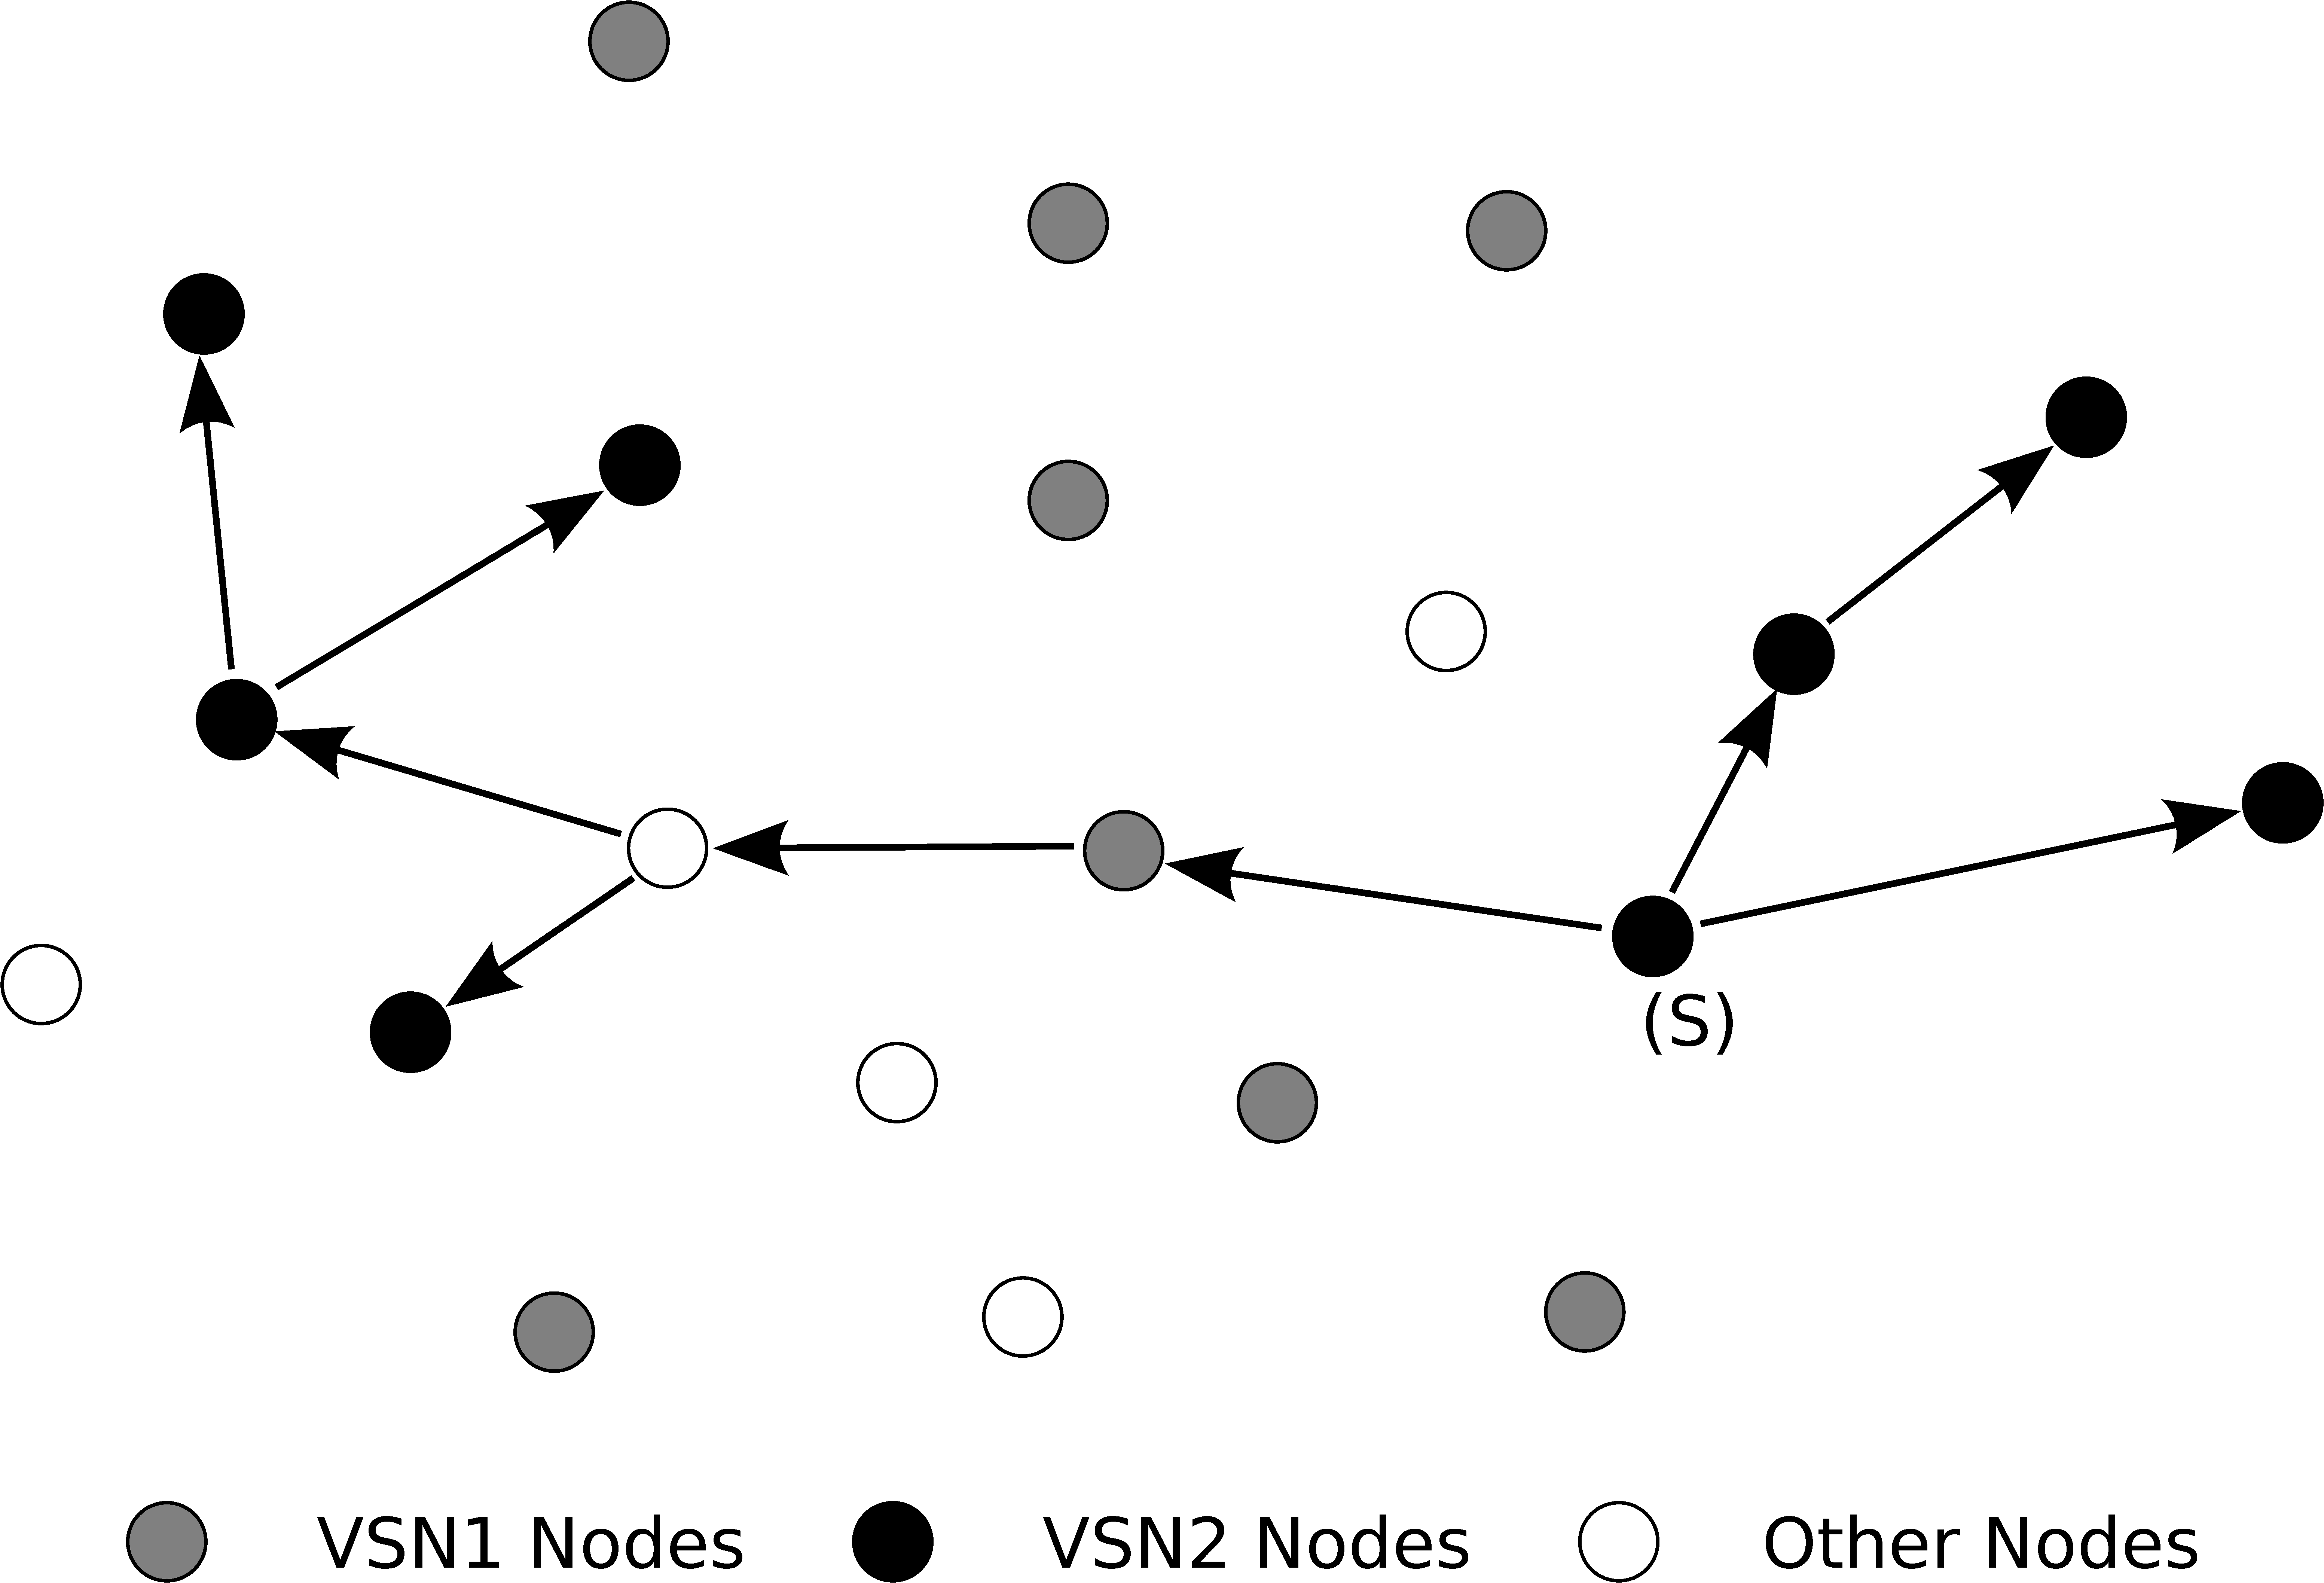
\includegraphics[width=3in]{figs/VirtualSensorNetwork.pdf}
 \caption{Broadcast path from a node (S) in VSN2.}
 \label{vsnfig}
\end{figure}


\subsubsection{Virtual Networks on Top of the Internet}
It is important to realize that the Internet, due to so many different participants with sometimes opposing interests, is hard to modify and only possible small and slow steps, if at all. Therefore, Virtual Networks are often the only way to realize innovation. To implement a Virtual Network using the existing Internet, several things need to be considered. First, the characteristics of the networking technology determine the attributes of the Virtual Network. For instance, a wired network yields a more scalable and bandwidth flexible Virtual Network than a wireless network would do. \cite{Chowdhury} Second, the layer of virtualization (referring to the OSI layer model) impacts the flexibility of the Virtual Network. That is, the lower the layer of virtualization, the more flexibility will be possible. Specifically, so-called overlay networks, mostly realized in the application layer, are limited in their ability to support fundamentally different architectures. \cite{Chowdhury} Moreover, virtualization on top of IP is fixed to the network layer protocol and cannot deploy IP independent mechanisms.  \cite{Chowdhury} Lastly, an important consideration in the non-comprehensive list is also about security and privacy in virtual networks. Thus, attack vectors such as denial-of-service or distributed denial-of-service against the underlying physical network will have impact on all simultaneously virtualized networks.
\subsubsection{Virtualization Algorithm}
Though, it is possible to form a VSN of mobile IoT devices by having access to all relevant data such as availability, sensor capabilities or sensor mobility, a more efficient solution is to assume the managing cloud agent does not have full knowledge of every sensors’ properties. \cite{Sherif} The cloud agent even may not be connected to all nodes but only to a subgroup of them. The presented algorithm also takes into account mobility of the devices which sometimes leads to nodes being unavailable for some time. \cite{Sherif}
This virtualization algorithm will search and select appropriate sensors from the whole network to form the virtual network which then executes the sensing task.


\subsection{WiFi Direct}
The goal of WiFi Direct technology is to improve direct device to device communications in Wi-Fi \cite{Mur}. The main strength of this technology is that it doesn’t require the presence of an Access Point \cite{Mur}. Actually direct device to device connection was already possible by the ad-hoc mode. But due to the power consumption issue, it is not popular \cite{Mur}. Instead WiFi Direct uses WiFi infrastructure mode \cite{Mur}. It let devices negotiate who will be the Access Point in this network \cite{Mur}. By doing so, it obtains all the enhanced QoS, power saving, and security mechanisms originally developed for the WiFi infrastructure mode \cite{Mur}. After first establish the network, new devices could connect to this network just like connecting to an Access Point \cite{Mur}.

\section{Solution}
To achieve the goals outlined in section~\ref{sec:problem} and implement them in ns-3, we took three vital steps.

\begin{itemize}
 \item Extend the Internet Control Message Protocol (ICMP) to support transmitting three simple control messages needed for our protocol.
 \item Develop a new application to be installed on network nodes. This application implements the gossip protocol.
 \item Import nodes information from a given topology file and export simulation results for performance evaluation.
\end{itemize}

\subsection{ICMP Extension}

ICMP stands for Internet Control Message Protocol. The most common use of ICMP is for error reporting~\cite{james}. ICMP message contains two parts: 8-byte header and data section. The first 4 btyes of the header have fixed format. However, the last 4 bytes various depend on the type or code of the ICMP packet~\cite{forouzan}. The first and second byte of the header is the type field and code field respectively. And the third and fourth byte are checksum field. The format of the header is shown in table \ref{table:1}.

\begin{table}[h!]
	\centering
	\caption{ICMP Header Structure}
	\label{table:1}
\begin{tabular}{|p{1 cm}|p{1 cm}|p{1 cm}|p{1 cm}|p{1 cm}|}
	\hline
	Octet & 0 & 1 & 2 & 3 \\
	\hline
	& Type & Code & 
	\multicolumn{2}{ |c| }{Checksum}  \\
	\hline
	Octet & 4 & 5 & 6 & 7 \\
	\hline
	& 
	\multicolumn{4}{|c|}{Rest of Header}  \\
	\hline
\end{tabular}
\end{table} 

Table \ref{table:2} here presented some selected ICMP message types. 

\begin{table}[h]
	\centering
	\caption{Control Messages}
	\label{table:2}
	\begin{tabular}{|p{1.5cm}|p{0.8 cm}|p{4.5 cm}|}
		\hline
		Type & Code & Description \\                                                           
		\hline
		0  & 0   & Echo reply   \\ \hline
		8  &  0 & Echo request \\ 
		\hline
		9 & 0 & Router Advertisement \\
		\hline
		10	& 0	&	Router discovery/selection/solicitation \\
		\hline
		42 to 255    &   & Reserved    \\ 
		\hline
	\end{tabular}
\end{table}

As we could see in table \ref{table:2}, type 42 to 255 are reserved for further development. So we decided to extend ICMP by defining type 42, 43, and 44 to represent ackownlegement, request, and data respectively. The detail is shown in table \ref{table:3}.

\begin{table}[h]
	\centering
	\caption{Gossip Protocol Control Messages}
	\label{table:3}
	\begin{tabular}{|p{0.8cm}|p{0.5 cm}|p{3.5 cm}|}
		\hline
		Type & Code & Description \\                                                           
		\hline
		42  & 0   & Send Acknowledgment   \\ \hline
		43  &  0 & Send Request \\ 
		\hline
		44 & 0 & Send Data \\
		\hline
	\end{tabular}
\end{table}

Upon these new control message types, we could further develop gossip protocol in ns-3.

\subsection{Gossip Protocol }

Gossip protocol is a computer communication protocol which inspired by the social activity -- gossip. This protocol accomplishes to synchronize a message in a system that does not need real-time synchronization. It provides $O(\log n)$ time to synchronize the message to the network, where $n$ means the number of nodes in the network. There are three packet types for the message protocol: Data packet, ACK packet and request packet. The data packet contains the message from a certain source node that wants to spread this message to the whole network. The ACK packet is a packet to notice the node that the destination already contains the message. The request packet is the packet that request the message from destination node. There are two states for each node, running and stop.

The pseudo code of gossip algorithm is given in figure~\ref{fig:pseudo}.

\begin{figure}
 \centering
 \begin{Verbatim}[fontsize=\small]
switch(state):
  case running:
    if message is not null:
      every 5 milliseconds:
        find a random neighbor R
        send data packet to R
      if receive a packet:
        if packet is ACK:
          state <- stop
        if packet is data:
          send ACK to packet source
    else:
      if receive a packet:
        if packet is a data packet:
          update the message
      every 5 seconds:
        find a random neighbor R
        send a request packet to R
        if receive a packet:
          if packet is a data packet:
            update the message to data
                    
  case stop:
    if receive a packet:
      if packet is request:
        send data to the source node
      if packet is data:
        send ACK to the source node
\end{Verbatim}
 \caption{The pseudo code of the gossip algorithm.}
 \label{fig:pseudo}
\end{figure}

The explanation of the pseudo code: 

All the node in network have same behavior and they are all independent. When we want to spread a message x to the whole network, we assign the x to message and run this algorithm. Node 1 start with running state, and node 1 has a message x, so it will find a random neighbor every five milliseconds and send a data packet which contain message x to its random neighbor. If node 1 receive a ACK packet it will go to stop state, otherwise it will keep doing these steps. Other nodes which do not have the message x will wait for packet, if a node 1 send a data packet to the node 2 which do not have message x, node 2 will update the message in node 2 and not return anything to node 1. If node 2 do not have message 2, it will send a request packet to a random neighbor every 5 second. If node 2 receives a data packet after sending the request packet, it will update its message to x. The nodes in stop state would always waiting for other node send message to it and it will send data packet or ACK packet back depends on what packet it receive.

\subsection{Gathering Simulation Data}

To evaluate the performance of the gossip protocol, we use several randomly generated topology files with the number of nodes as variable. Those topology files are derived from a random geometric graph network, which was created by uniformly and randomly placing nodes into a space and then connect nodes whose distance is smaller than some given radius.

\begin{figure}
 \centering
 \begin{Verbatim}[fontsize=\small]
#Nodes
0
1
2
#Edges
(0, 1)
(1, 2)
\end{Verbatim}
 \caption{A topology file of a linear topology with three nodes.}
 \label{fig:topsimple}
\end{figure}


Each topology file contains the number of nodes as well as all the edges, which are connections between nodes. As an example, the content of a simple topology file is shown in figure~\ref{fig:topsimple}. We assumed in our work, that each nodes is connected at least once to the network. We wrote a parser in C++ to create the given number of nodes in ns-3 and installed the gossip protocol application on them. Thereafter, all edges are parsed and created accordingly. Each node holds an ns-3 Ipv4Interface for every connection and stores the address of his interface and the one of his neighbors interface.

For our simulation, we set the link rate for all connections to 100~Mbps and the link delay to 2~ms. Also, all nodes are instructed to execute the gossip process of sending out data periodically every 5~ms. The interval of requesting new data is set to 5~s.

To allow the performance analysis, all nodes count the number of ICMP messages they sent. Also, they track how many hops the data message experienced before reaching them and they record the time when they received the data message. For one single simulation, we collect the information from the nodes and determine the average amount of ICMP messages sent. Moreover, the highest number of reported hops is saved, as well as how long it took for the message to reach the ``last'' node.

This information is determined and stored for each of the several hundred topology files. It should be noted that due to time limitations each topology file was only simulated once. Finally, we did statistical analysis upon those collected data in the hope of verifying the assumptions we made in section~\ref{sec:problem}.

\section{Performance Evaluation}
The random generated topology files are the input of our simulations. There are 11 different cases where the number of nodes vary from 100 to 1600 , increasing with 150 nodes step. And for each case, we u


First, we will have a look at the average number of ICMP messages each node sent, depicted in fig.~\ref{fig:avgmsg}. It is important to note that the the collected average number for one topology file was again averaged over all reported values produced by topology files with the same number of nodes. Thus, the error bar is an indicator how consistent the average number is. It can be deduced from fig.~\ref{fig:avgmsg} that this value is a constant roughly equal to 3.3. Only when a very litte number of nodes is observed, the mean and variance of the average amount of sent messages increases.
%\textcolor{red}{Is this a fluctuation or can this be ``normalized'' by running the simulation for each topology file a lot more often?}

\begin{figure}
	\centering
	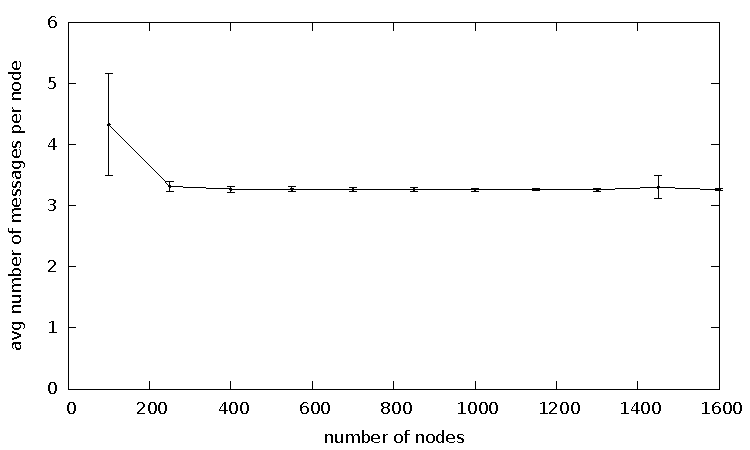
\includegraphics[width=3in]{figs/avgmsg}
	\caption{The average number of messages each node sent over the duration of a whole simulation.}
	\label{fig:avgmsg}
\end{figure}

Second, the maximum number of hops a message experiences is analyzed. Figure~\ref{fig:maxhops} shows that with a growing number of nodes, the average maximum hops slightly increases as well. But the standard deviation has the tendency to decrease which is a positive sign since we hope the gossip protocol performance metrics would converge as the network grows. Nonetheless, the overall impression is that the number of hops is generally speaking, more or less constant and mostly is found to range from 15 to 20. 

\begin{figure}
	\centering
	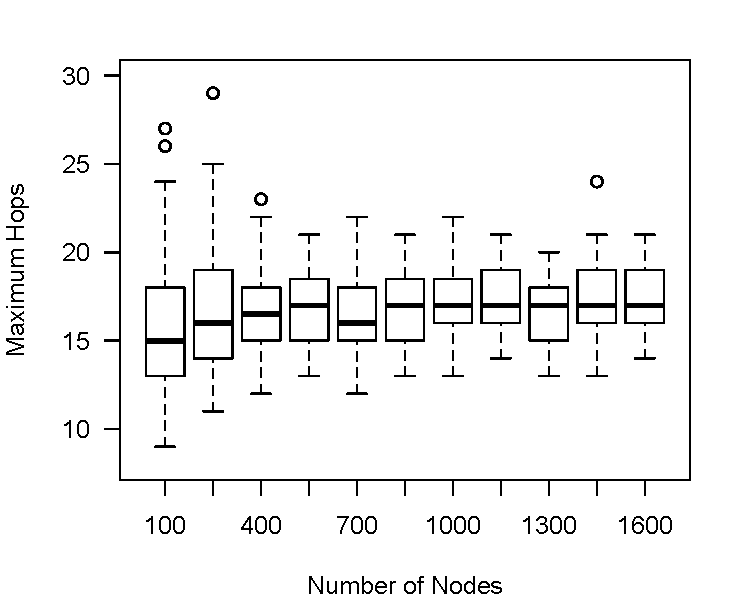
\includegraphics[width=3in]{figs/bpHopsNodes}
	\caption{The maximum amount of hops the message experienced over the duration of a whole simulation.}
	\label{fig:maxhops}
\end{figure}

Moreover, figure~\ref{fig:maxtime} illustrates the time needed to spread the message across the whole network. Again, the mean is found to be more or less constant and slightly less than 15~s. Due to the huge difference in the gossip-interval-time (5~ms) and solicit-interval-time (5~s), only the influence of the solicit-interval can be deduced from the results. One can see, that the time needed to spread the message is fluctuating due to the random nature of the gossip protocol, especially for the case of a number of nodes of 100, where the standard deviation is the largest.

\begin{figure}
	\centering
	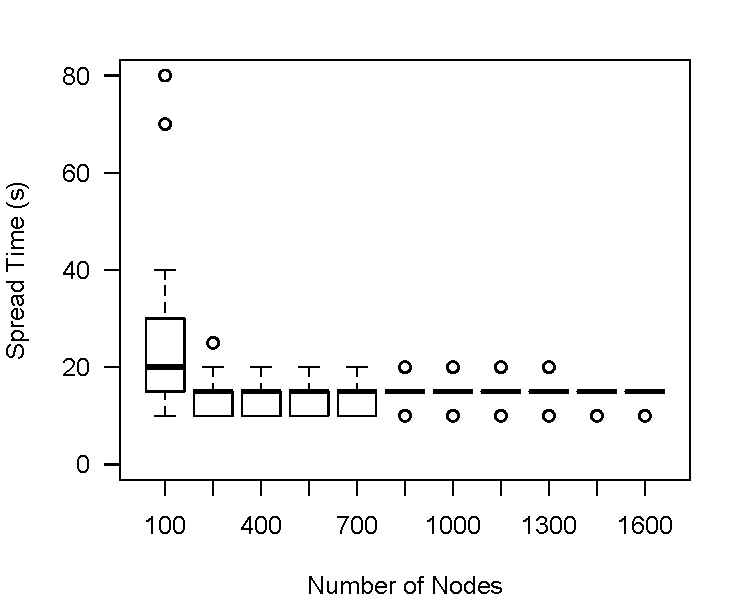
\includegraphics[width=3in]{figs/bpTimeNodes}
	\caption{The spread time under different number of nodes cases}
	\label{fig:maxtime}
\end{figure}

We assume that the reason that the results being not a function of the number of the nodes but rather seem more or less constant, is due to the increasing edge density with higher numbers of nodes. As seen in fig.~\ref{fig:density}, the number of edges is strictly linear depending only on the number of nodes in the topology. We also consider this as the reason we could not verify the logarithmic complexity suggested by \cite{gossip}.

\begin{figure}
	\centering
	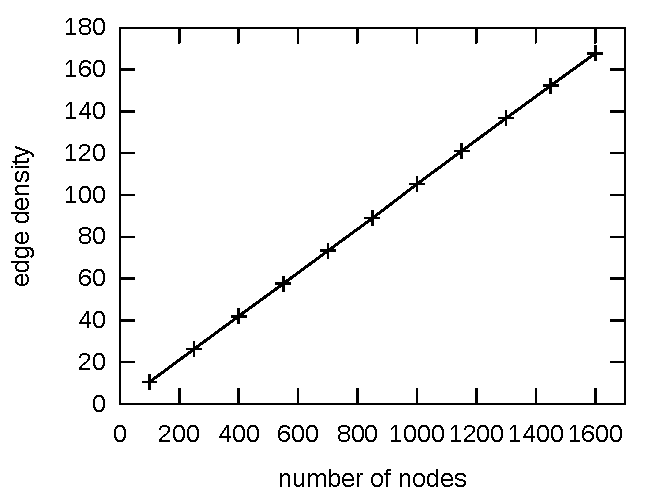
\includegraphics[width=3in]{figs/density}
	\caption{The density of the nodes for each batch of topology files.}
	\label{fig:density}
\end{figure}

Another interesting observation is that accross these statistical analysis, the case of 100 nodes 

Section~\ref{sec:further} proposes further work which can be done to gain a more thorough evaluation.

\section{Conclusion}
We introduced the topics of Internet of things and sensor networks. The opportunities resulting by virtualization of those sensor networks have been elaborated. A distributed algorithm to spread data across a mesh-network has been implemented. We proposed several performance measures to evaluate this algorithm.

We have implemented the gossip protocol and run the simulation in ns-3. The result from ns-3 shows that the number of messages a node expects to send is not a function of the total number of nodes in the network. Further, we see that the maximum number of hops is slightly increasing for an increasing number of nodes. And lastly, our results imply that the time until all nodes have the data, is mostly only depended on how the solicit-interval is chosen.Unfortunately, we could not verify that the time complexity of the algorithm is $O(\log n)$ as outlined in \cite{gossip}. Possible causes to consider are discussed in the next section.

\section{Further Work}\label{sec:further}
In further work, various alterations to the gossip protocol can be covered and examined. For example, a node can improve routing (or decrease the number of hops) by notifying neighbors if there exists a shorter route to the owner of a message. To accomplish this, they need to keep track of the number of hops and then compare if the owner of a received message is one of their immediate neighbors. In case this is true and they will notify the source of the message, that the \textit{true} (or ideal) number of hops would be 1.

Another option for further work, would be to change the parameters to create the topology file. As demonstrated in fig.~\ref{fig:density}, the number of edges per node is not a constant. We believe that making this value constant, will yield different results which possibly verify the logarithmic complexity suggested by \cite{gossip}.

And lastly, the effect of reducing the solicit interval should be investigated. Clearly, having a faster rate to request new data will add an overhead to the network. Further work may determine an appropriate interval for the solicit interval.

Due to time limitations we could not address the huge spectrum of possible analysis. Further work is needed to examine the effects when the wired peer-to-peer links between nodes are replaced by wireless ones. Power limitations and mobility of the nodes should be included in such a scenario. Thus, the list of neighbors for each node changes over time and a topology file is not needed anymore. In the wireless case, Wi-Fi Direct can be used to connect devices with each other as well.



% if have a single appendix:
%\appendix[Proof of the Zonklar Equations]
% or
%\appendix  % for no appendix heading
% do not use \section anymore after \appendix, only \section*
% is possibly needed

% use appendices with more than one appendix
% then use \section to start each appendix
% you must declare a \section before using any
% \subsection or using \label (\appendices by itself
% starts a section numbered zero.)
%



% use section* for acknowledgment
\section*{Acknowledgment}
We would like to thank Dr. Bechir Hamdaoui for his advising. We also would like to thank Sherif Abelwahab for providing useful information and answers to our questions in numerous discussions. In addition, our team would like to thank Kendall Bailey for her suggestion about automating simulation process.

%The authors would like to thank...


% Can use something like this to put references on a page
% by themselves when using endfloat and the captionsoff option.
\ifCLASSOPTIONcaptionsoff
  \newpage
\fi

% trigger a \newpage just before the given reference
% number - used to balance the columns on the last page
% adjust value as needed - may need to be readjusted if
% the document is modified later
%\IEEEtriggeratref{8}
% The "triggered" command can be changed if desired:
%\IEEEtriggercmd{\enlargethispage{-5in}}

% references section

% can use a bibliography generated by BibTeX as a .bbl file
% BibTeX documentation can be easily obtained at:
% http://www.ctan.org/tex-archive/biblio/bibtex/contrib/doc/
% The IEEEtran BibTeX style support page is at:
% http://www.michaelshell.org/tex/ieeetran/bibtex/

% argument is your BibTeX string definitions and bibliography database(s)
%\bibliography{IEEEabrv,../bib/paper}
%
% <OR> manually copy in the resultant .bbl file
% set second argument of \begin to the number of references
% (used to reserve space for the reference number labels box)

\bibliography{mybib}{}
\bibliographystyle{ieeetr}

\appendices
\section{Division of Responsibilities}
Our team of three members had different responsibilities in fullfilling the project's goal. All of us did reasearch in the field of IoT, Sensor Networks and distributed algorithms. Each of us wrote different sections of the paper and helped improving all other sections by proof-reading.

The two graduate students -- Marco Falke and Tingzhi Li -- wrote the section about related work. Marco Falke wrote about Virtual Networks and Tingzhi Li covered WiFi Direct.

The different coding parts were assigned as follows. Jinming Mu did the initial setup of ns-3 and coded the topology creationg part of the code. Marco Falke had the responsibility to implement the Gossip protocol in form of a ns-3 application. Furthermore, he wrote the topology file parser to read a given topology file. Lastly, he coded the connection between the ICMP level of ns-3 and application level. Tingzhi Li did modifications to the ICMP part of ns-3 to allow transmission of modified control messages. Moreover, he wrote code to process the produced data and create plots.

%... Please add stuff that I was missing. Hardly remember the things. ;) --Marco

\end{document}


